% !TEX root = ../root.tex

\chapter{Splines on Lie Groups}

\begin{figure}[h]
  \begin{center}
    \begin{tikzpicture}
      \foreach \n in {0,1,2,...,10}
        {
          \coordinate (T\n) at ($(0,0)+(\n*1cm,0)$) {};
          \draw ($(T\n)+(0,5pt)$) -- ($(T\n)-(0,5pt)$);
          \node at ($(T\n)-(0,3ex)$) {$t_{\n}$};
          \coordinate (P\n) at ($(0,2)+(\n*1cm,{sin(\n r)})$) {};
          \node at (P\n)[circle, fill, inner sep=1.5pt] {};
          \node at ([yshift=-5mm]P\n) {$\x_{\n}$};
        }
      \draw[-latex] (T0) -- (T10) -- ($(T10)+1.5*(1,0)$);
    \end{tikzpicture}
  \end{center}
\end{figure}

It is often convenient to be able to interpolate sparsely defined data. Examples in robotics include representing trajectories as a sequence of $(t_{i}, \x_{i})$ pairs, and interpolating sensor data for calibration.

A general form for a spline $p(x)$ constructed from \emph{control points} $\x_{i}$ is
\begin{equation}
  \label{eq:spline}
  p(t) = \sum_{i=0}^{n} B_{i}(t) \x_{i},
\end{equation}
where $\B_{i}$ are some form of \emph{basis functions} that form a partition of unity, i.e. $\sum_{i} B_{i} (t) = 1$ for all $t$. The weighted sum does not have an immediate analogue on Lie groups, but \eqref{eq:spline} can be re-arranged on \emph{cumulative form} as
\begin{equation}
  \label{eq:cum_spline}
  p(t) = \x_{0} + \sum_{i=1}^{n} \tilde B_{i}(t) (\x_{i} - \x_{i-1}),
\end{equation}
where $\tilde B_{i}(t) = \sum_{j=i}^{n} B_{i}(t)$ are \emph{cumulative basis functions}. From this formulation we can write down a Lie group generalization as follows:
\begin{equation}
  \label{eq:cum_spline_liegroup}
  p(t) = \x_{0} \circ \exp \left(\tilde B_{1}(t) (\x_{1} \ominus \x_{0}) \right) \circ \exp \left(\tilde B_{2}(t) (\x_{2} \ominus \x_{1}) \right) \circ \ldots \circ \exp \left(\tilde B_{n}(t) (\x_{n} \ominus \x_{n-1}) \right)
\end{equation}

We first discuss two choices for basis functions---Bezier curves and B-Splines---and then show how the value and derivatives of such splines can be calculated.

Below we will need the derivative with respect to $t$ of \eqref{eq:cum_spline_liegroup}. For this purpose it will be convenient to introduce the variables
\begin{equation}
  \begin{aligned}
    \symbf v_{i} = \x_{i} \ominus \x_{i-1}, \\
    \symbf s_{i} = \tilde B_{i}(t) \symbf v_{i}.
  \end{aligned}
\end{equation}
With this notation, $\mathrm{d}^{r} \left( \exp \symbf s_{i} \right)_{t} = \tilde B_{i}'(t) \mathrm{d}^{r} \exp_{\symbf s_{i}} \symbf v_{i} = \tilde B_{i}'(t) \symbf v_{i}$. We can now write down the derivative of \eqref{eq:cum_spline_liegroup} by utilizing \eqref{eq:d_composition_rght_fst} and \eqref{eq:d_composition_rght_snd}:
\begin{equation}
  \label{eq:cum_spline_liegroup_deriv}
  \begin{aligned}
    \mathrm{d}^{r} p_{t} & = \bAd_{\exp(-\symbf s_{n})} \mathrm{d}^{r} \left( \x_{0} \exp(\symbf s_{1})  \ldots \exp(\symbf s_{n-1})\right)_{t} + \mathrm{d}^{r} \exp (\symbf s_{n})_{t}                                                                              \\
                         & = \bAd_{\exp(-\symbf s_{n}) \exp(-\symbf s_{n-1})} \mathrm{d}^{r} \left( \x_{0} \exp(\symbf s_{1})  \ldots \exp(\symbf s_{n-2})\right)_{t} + \bAd_{\exp(-s_{n})} \mathrm{d}^{r} \exp (\symbf s_{n-1})_{t} + \mathrm{d}^{r} \exp(s_{n})_{t} \\
                         & = \sum_{i=1}^{n} \bAd_{\exp(-\symbf s_{n}) \ldots \exp(-\symbf s_{i+1})} \mathrm{d}^{r} \exp (\symbf s_{i})_{t} = \sum_{i=1}^{n} \tilde B_{i}'(t) \bAd_{\exp(-\symbf s_{n}) \ldots \exp(-\symbf s_{i+1})} \symbf v_{i}.
  \end{aligned}
\end{equation}

\section{Bezier Curves}

\begin{figure}[h]
  \begin{center}
    \footnotesize
    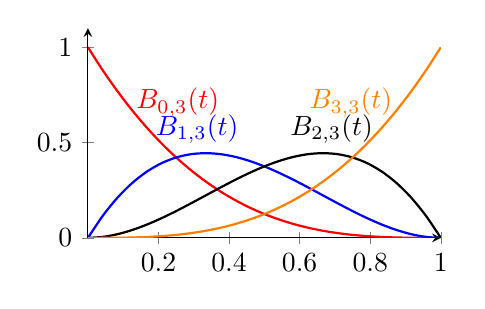
\begin{tikzpicture}[]
      \begin{axis}[
          axis y line=left,
          axis x line=middle,
          width=0.5\columnwidth,
          height=0.35\columnwidth,
          xmin=0,
          xmax=1,
          ymin=-0.,
          ymax=1.1
        ]
        \addplot+[red, no marks, thick, smooth, domain=0:1] ({\x}, {(1-3*\x+3*\x^2-\x^3)}) node[pos=0.2, right] {$B_{0,3}(t)$};
        \addplot+[blue, no marks, thick, smooth, domain=0:1] ({\x}, {(3*\x-6*\x^2+3*x^3)}) node[pos=0.4, above] {$B_{1,3}(t)$};
        \addplot+[black, no marks, thick, smooth, domain=0:1] ({\x}, {(3*\x^2-3*\x^3)}) node[pos=0.6, above] {$B_{2,3}(t)$};
        \addplot+[orange, no marks, thick, smooth, domain=0:1] ({\x}, {(x^3)}) node[pos=0.8, left] {$B_{3,3}(t)$};
      \end{axis}
    \end{tikzpicture}~
    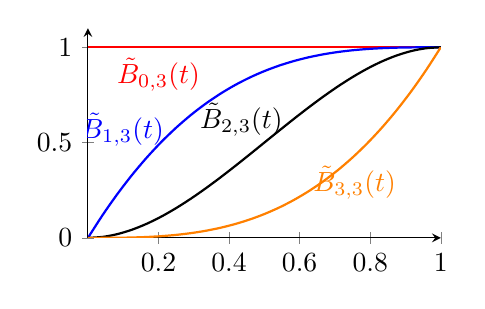
\begin{tikzpicture}[]
      \begin{axis}[
          axis y line=left,
          axis x line=middle,
          width=0.5\columnwidth,
          height=0.35\columnwidth,
          xmin=0,
          xmax=1,
          ymin=-0.,
          ymax=1.1
        ]
        \addplot+[red, no marks, thick, smooth, domain=0:1] ({\x}, {(1)}) node[pos=0.2, below] {$\tilde B_{0,3}(t)$};
        \addplot+[blue, no marks, thick, smooth, domain=0:1] ({\x}, {(3*\x-3*\x^2+x^3)}) node[pos=0.4, left] {$\tilde B_{1,3}(t)$};
        \addplot+[black, no marks, thick, smooth, domain=0:1] ({\x}, {(3*\x^2-2*\x^3)}) node[pos=0.6, left] {$\tilde B_{2,3}(t)$};
        \addplot+[orange, no marks, thick, smooth, domain=0:1] ({\x}, {(x^3)}) node[pos=0.6, below] {$\tilde B_{3,3}(t)$};
      \end{axis}
    \end{tikzpicture}
  \end{center}
  \caption{Bernstein cubic (order 3) basis functions (left) and cumulative basis functions (right).}
  \label{fig:bezier}
\end{figure}

A Bezier curve of order $k$ is defined on the interval $[0, 1]$ via the \emph{Bernstein basis functions} defined as
\begin{equation}
  B_{i, k}(t) = \binom{k}{i} t^{i} (1 - t)^{k - i}, \qquad i = 0, \ldots, k.
\end{equation}
The binomial formula $1 = (t + 1 - t)^{n} = \sum_{i=0}^{n}B_{i, k}(t)$ shows that the Berstein basis is indeed a partition of unity. A Bezier spline is a curve that consists of Bezier curve pieces.

The Bernstein basis functions have the following properties
\begin{itemize}
  \item They satisfy the recurrence relation
        \begin{equation}
          \label{eq:bezier_recurrence}
          B_{i, k}(t) = t B_{i-1, k-1}(t) + (1-t) B_{i, k-1}(t).
        \end{equation}
  \item They are symmetric in the sense that $B_{i, k}(t) = B_{k-i, k}(1 - t)$.
  \item The derivative can be expressed in terms of lower-order polynomials
        \begin{equation*}
          \begin{aligned}
            B_{i, k}'(t)
             & = i \binom{k}{i} t^{i-1} (1-t)^{k-i} - (k-i) \binom{k}{i} t^{i} (1-t)^{k-i-1}                                                                         \\
             & = \frac{k!}{(i-1)! (k-i)!} t^{i-1} (1-t)^{k-i} + \frac{k!}{i! (k-i-1)!} t^{i} (1 - t)^{k - i + 1} = k \left(  B_{i-1, k-1}(t) - B_{i, k-1}(t)\right).
          \end{aligned}
        \end{equation*}
  \item At $t = 0$ only the first spline is nonzero: $B_{0, k}(0) = 1$, and $B_{1, k}(0) = \ldots = B_{k, k}(0) = 0$. It follows that the non-zero derivatives at $t = 0$ are $B_{0, k}'(0) = -k$ and $B_{1, k}'(0) = k$. The converse holds for $t = 1$ due to symmetry.
  \item At $t = 0$ only the $i=0$ cumulative spline is nonzero: $\tilde B_{0, k}(0) = 1$, and only the $i=1$ cumulative derivative is non-zero: $\tilde B_{1, k}'(0) = k$.
  \item At $t = 1$ only the $i=k$ cumulative spline is nonzero: $\tilde B_{k, k}(1) = 1$, and only the $i=k$ cumulative derivative is non-zero: $\tilde B_{k, k}'(0) = k$.
\end{itemize}

Utilizing these fact and that $\mathrm{d}^{r} \exp_{\a} \a = \a$ we can evaluate \eqref{eq:cum_spline_liegroup} and \eqref{eq:cum_spline_liegroup_deriv}
\begin{equation}
  p(0) = \x_{0}, \quad p(1) = \x_{n}, \quad \left. \mathrm{d}^{r} p_{t} \right|_{t=0} = \tilde B_{1, k}'(0) \symbf v_{1} = k \symbf v_{1}, \quad
  \left. \mathrm{d}^{r} p_{t} \right|_{t=1} = \tilde B_{k, k}'(0) \symbf v_{k} = k \symbf v_{k}.
\end{equation}
These formulas can be used to fit low-degree splines to given boundary conditions.

\subsection{Quadratic Bezier curve} A $k=2$ spline $\x(t) = \x_{0} \exp \left( \tilde B_{1, 2}(t) \symbf v_{1}\right) \exp\left(\tilde B_{2, 2}(t) \symbf v_{2}\right)$ such that $\x(0) = \x_{a}, \x(1) = \x_{b}$, and $\left. \mathrm{d}^{r} \x_{t} \right|_{t=0} = \a_{a}$ is defined by the coefficients
\begin{equation}
  \x_{0}  = \x_{a}, \quad
  \symbf v_{1} = \frac{\a_{a}}{2}, \quad  \symbf v_{2} = \log \left( \exp \left( -\frac{\a_{a}}{2} \right) \x_{a}^{-1} \x_{b} \right),
\end{equation}
and has the property that $\left. \mathrm{d}^{r} \x_{t} \right|_{t=1} = 2 \symbf v_{2}$.

\subsection{Cubic Bezier curve} For the cubic case $k = 3$ a Bezier curve takes the form
\begin{equation}
  \x(t) = \x_{0} \exp \left( \tilde B_{1, 3}(t) \symbf v_{1}\right) \exp\left(\tilde B_{2, 3}(t) \symbf v_{2}\right)\exp\left(\tilde B_{3, 3}(t) \symbf v_{3}\right)
\end{equation}
and has first and second derivatives w.r.t. time
\begin{equation}
  \begin{aligned}
    \mathrm{d}^{r }\x_{t}  & = \tilde B_{1, 3}'(t) \bAd_{\exp (-\symbf s_{3})} \bAd_{\exp(-\symbf s_{2})} \symbf v_{1}                                                                                         \\
                           & + \tilde B_{2, 3}'(t) \bAd_{\exp (-\symbf s_{3})} \symbf v_{2}                                                                                                                    \\
                           & + \tilde B_{3, 3}'(t) \symbf v_{3}                                                                                                                                                \\
    \mathrm{d}^{2r}\x_{tt} & = \tilde B_{1, 3}''(t) \bAd_{\exp (-\symbf s_{3})} \bAd_{\exp(-\symbf s_{2})} \symbf v_{1}                                                                                        \\
                           & \quad - \tilde B_{1,3}'(t) \tilde B_{3, 3}'(t) \left[ \symbf v_{3}, \bAd_{\exp(-\symbf s_{3})} \bAd_{\exp(-\symbf s_{2})} \symbf v_{1} \right]                                    \\
                           & \quad - \tilde B_{1,3}'(t) \tilde B_{2, 3}'(t) \bAd_{\exp(-\symbf s_{3})} \left[ \symbf v_{2}, \bAd_{\exp(-\symbf s_{2})} \symbf v_{1} \right ]                                   \\
                           & + \tilde B_{2, 3}''(t) \bAd_{\exp (-\symbf s_{3})} \symbf v_{2} - \tilde B_{2, 3}'(t) \tilde B'_{3, 3}(t) \left[ \symbf v_{3} , \bAd_{\exp(- \symbf s_{3})} \symbf v_{2} \right ] \\
                           & + \tilde B_{3, 3}''(t) \symbf v_{3}.
  \end{aligned}
\end{equation}
The cumulative basis functions of order three are $\tilde B_{1, 3}(t) = 3t - 3 t^{2} + t^{3}$, $\tilde B_{2, 3}(t) = 3x^{2} - 2 x^{3}$, and $\tilde B_{3, 3}(t) = t^{3}$. With the derivative formulas above it therefore follows that
\begin{equation}
  \begin{aligned}
    \left. \mathrm{d}^{r} \x_{t} \right|_{t = 0}   & = 3 \symbf v_{1}, \quad \left. \mathrm{d}^{r} \x_{t} \right|_{t = 1} = 3 \symbf v_{3},                                                                            \\
    \left. \mathrm{d}^{2r} \x_{tt} \right|_{t = 0} & = 6 (\symbf v_{2} - \symbf v_{1}), \quad \left. \mathrm{d}^{2r} \x_{tt} \right|_{t = 1} = 6 \left(\symbf v_{3} - \bAd_{\exp(-\symbf v_{3})} \symbf v_{2} \right)
  \end{aligned}
\end{equation}
This information can be used in two ways.

\paragraph{Bezier curve with given endpoint velocities} First, if the values $\x_{a}, \x_{b}$ and first-order derivatives $\a_a, \a_{b}$ at the end points are given there is a unique Bezier curve $\x(t)$ such that $\x(0) = \x_{a}, \x(1) = \x_{b}, \left. \mathrm{d}^{r} \x_{t} \right|_{t = 0} = \a_{a}$, and $\left. \mathrm{d}^{r} \x_{t} \right|_{t = 1} = \a_{b}$. It is defined by the coefficients
\begin{equation}
  \x_{0}  = \x_{a}, \quad
  \symbf v_{1} = \frac{\a_{a}}{3}, \quad  \symbf v_{3} = \frac{\a_{b}}{3}, \quad  \symbf v_{2} = \log \left( \exp \left( -\frac{\a_{a}}{3} \right) \x_{a}^{-1} \x_{b} \exp \left( -\frac{\a_{b}}{3} \right ) \right).
\end{equation}

\paragraph{Cubic interpolating Bezier spline} Secondly, an interpolating spline for a dataset $\{ ( t_{i}, \x_{i} ) \}_{i=0}^{n}$ can be defined as a collection of $n$ Bezier curves $$\x_{i}(u) = \x_{a, i} \exp (\tilde B_{1, 3}(u) \symbf v_{1, i})\exp (\tilde B_{2, 3}(u) \symbf v_{2, i})\exp (\tilde B_{3, 3}(u) \symbf v_{3, i})$$ where $u = (t - t_{i}) / (t_{i+1} - t_{i}) \in [0, 1]$. To ensure a smooth interpolation consider the following constraints (for simplicity we assume that $t_{i+1} - t_{i} = 1$ for all $i$; if not the derivative constraints have to be rescaled):
\begin{itemize}
  \item Interpolation: $\x_{a, i} = \x_{i}$ and $\x_{a, i} \exp(\symbf v_{1}) \exp(\symbf v_{2})\exp(\symbf v_{3})= \x_{i+1}$, for $i = 0, \ldots, n-1$,
  \item First derivative continuity: $\symbf v_{3, i} = \symbf v_{1, i+1}$ for $i = 0, \ldots, n-2$,
  \item Second derivative continuity: $\bAd_{\exp(-\symbf v_{3, i})} \symbf v_{2, i} - \symbf v_{3, i} = \symbf v_{2, i+1} - \symbf v_{1, i+1}$ for $i = 0, \ldots, n-2$,
  \item Zero second derivative at start: $\symbf v_{2, 0} - \symbf v_{1, 0} = 0$, and at end: $\bAd_{\exp(-\symbf v_{3, n-1})} \symbf v_{2, n-1} - \symbf v_{3, n-1} = 0$.
\end{itemize}
The variables $\x_{a, i}, \x_{b, i}$ can be eliminated to end up with the following system of equations for $\symbf v_{j, i}$:
\begin{equation}
  \label{eq:cubic_spline_equations}
  \begin{aligned}
     & \symbf v_{2, 0} = \symbf v_{1, 0},                                                                                                   \\
     & \bAd_{\exp(-\symbf v_{3, n-1})}\symbf v_{2, n-1} = \symbf v_{3, n-1},                                                                \\
     & \exp (\symbf v_{1, i}) \exp (\symbf v_{2, i}) \exp (\symbf v_{3, i}) = \x_{i}^{-1} \x_{i+1},                      & \quad i = 0, \ldots, n-1, \\
     & \symbf v_{3, i} = \symbf v_{1, i+1},                                                                     & \quad i = 0, \ldots, n-2, \\
     & \bAd_{\exp(-\symbf v_{3, i})} \symbf v_{2, i} - \symbf v_{3, i} = \symbf v_{2, i+1} - \symbf v_{1, i+1}, & \quad i = 0, \ldots, n-2. \\
  \end{aligned}
\end{equation}
For Euclidean space this is a linear system of equations and is therefore straightforward to solve, but on Lie groups this is no longer possible due to nonlinearities. To find an interpolating spline we therefore either have to solve a nonlinear system of equations, or give up the strict requirement on continuity of the second-order derivatives. The following simple algorithm is of the latter kind:
\begin{enumerate}
  \item Solve the following linearized version of \eqref{eq:cubic_spline_equations}:
        \begin{equation}
          \label{eq:cubic_spline_equations_linearized}
          \begin{aligned}
             & \symbf v_{2, 0} = \symbf v_{1, 0},                                                                               \\
             & \symbf v_{2, n-1} = \symbf v_{3, n-1},                                                                           \\
             & \symbf v_{1, i} + \symbf v_{2, i} + \symbf v_{3, i} = \log\left(\x_{i}^{-1} \x_{i+1} \right), & \quad i = 0, \ldots, n-1, \\
             & \symbf v_{3, i} = \symbf v_{1, i+1},                                                 & \quad i = 0, \ldots, n-2, \\
             & \symbf v_{2, i} - \symbf v_{3, i} = \symbf v_{2, i+1} - \symbf v_{1, i+1},           & \quad i = 0, \ldots, n-2. \\
          \end{aligned}
        \end{equation}
  \item Set $\symbf v_{2, i} = \log \left( \exp(-\symbf v_{1, i}) x_{i}^{-1} x_{i+1} \exp(-\symbf v_{3, i}) \right )$ for $i = 0, \ldots, n-1$.
\end{enumerate}
The first step finds values for all coefficients that do not necessarily produce a continuous spline. This is however rectified in the second step. The resulting spline is guaranteed to be continuous and have a continuous first-order derivative, but in general does not have a continuous second-order derivative.

\section{B-Splines}

\begin{figure}[h]
  \begin{center}
    \footnotesize
    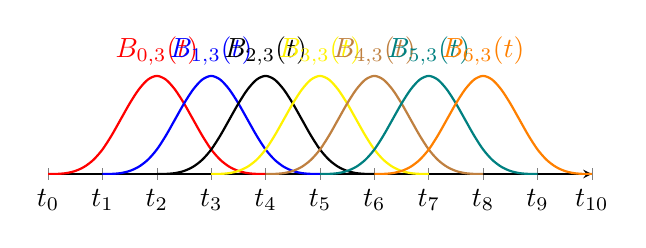
\begin{tikzpicture}[
        declare function={
            bspline3(\x) = and(0<=\x, \x<1) * (\x^3/6) +
            and(1<=\x, \x<2) * ((-3*(\x-1)^3+3*(\x-1)^2+3*(\x-1)+1)/6) +
            and(2<=\x, \x<3) * ((3*(\x-2)^3-6*(\x-2)^2+4)/6) +
            and(3<=\x, \x<4) * ((-(\x-3)^3+3*(\x-3)^2-3*(\x-3)+1)/6);
          }
      ]
      \begin{axis}[
          axis y line=none,
          axis x line=middle,
          xtick={0, 1, 2, 3, 4, 5, 6, 7, 8, 9, 10},
          xticklabels={$t_0$, $t_1$, $t_2$, $t_3$, $t_4$, $t_5$, $t_6$, $t_7$, $t_8$, $t_9$, $t_{10}$},
          width=0.7\columnwidth,
          height=0.3\columnwidth,
          xmin=0,
          xmax=10,
          ymin=-0.,
          ymax=1.1,
          cycle list name=color list]
        \pgfplotsinvokeforeach {0, 1, 2, 3, 4, 5, 6} {
          \addplot+[no marks, thick, smooth, domain=#1:#1+4] ({\x}, {bspline3(\x-#1)}) node[pos=0.5, above] {$B_{#1,3}(t)$};
        }
      \end{axis}
    \end{tikzpicture} \\
    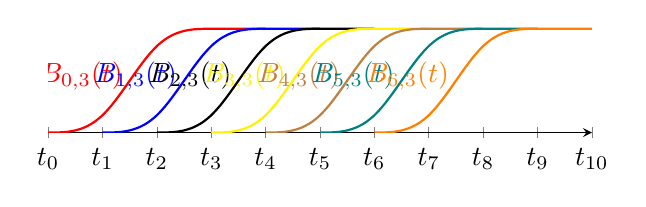
\begin{tikzpicture}[
        declare function={
            cbspline3(\x) = and(0<=\x, \x<1) * ((\x^3                                          )/6) +
            and(1<=\x, \x<2) *                 ((-2*(\x-1)^3  + 3*(\x-1)^2    +3*(\x-1)       +1)/6) +
            and(2<=\x, \x<3) *                 ((1*(\x-2)^3   - 3*(\x-2)^2    +3*(\x-2)       +5)/6) +
            and(3<=\x, \x<4) *                 ((0*(\x-3)^3   + 0*(\x-3)^2    +0*(\x-3)       +6)/6);
          }
      ]
      \begin{axis}[
          axis y line=none,
          axis x line=middle,
          xtick={0, 1, 2, 3, 4, 5, 6, 7, 8, 9, 10},
          xticklabels={$t_0$, $t_1$, $t_2$, $t_3$, $t_4$, $t_5$, $t_6$, $t_7$, $t_8$, $t_9$, $t_{10}$},
          width=0.7\columnwidth,
          height=0.25\columnwidth,
          xmin=0,
          xmax=10,
          ymin=-0.,
          ymax=1.1,
          cycle list name=color list]
        \pgfplotsinvokeforeach {0, 1, 2, 3, 4, 5, 6} {
          \addplot+[no marks, thick, smooth, domain=#1:#1+4] ({\x}, {cbspline3(\x-#1)}) node[pos=0.4, left] {$B_{#1,3}(t)$};
        }
      \end{axis}
    \end{tikzpicture}
  \end{center}
  \caption{B-spline basis function and cumulative basis functions. For $k=3$ and $t \in [t_4, t_5)$ the non-zero basis functions are $B_{1, 4}, B_{2, 4}, B_{3, 4}$ and $B_{4, 4}$.}
  \label{fig:bspline_nonzero}
\end{figure}

A B-spline interpolation of order $k$ is a function $\x(t) = \sum_{i=0}^N B_{i, k}(t) \x_{v(i)}$ where $\x_{v(i)} \in \mathbb{R}^n$ are \textbf{control points} for \textbf{knots} $t_i$, and $B_{i, k}(t)$ are \textbf{basis functions} recursively defined as

\begin{equation}
  \label{eq:b_spline_rec}
  \begin{aligned}
    B_{i, 0}(t) & = \begin{cases}
      1 & t_i \leq t < t_{i+1}, \\
      0 & \text{otherwise}.
    \end{cases}                                                                               \\
    B_{i, k}(t) & = \frac{t - t_i}{t_{i+k} - t_i} B_{i, k-1}(t) + \frac{t_{i+k+1} - t}{t_{i+k+1} - t_{i+1}} B_{i+1, k-1}(t).
  \end{aligned}
\end{equation}

The following are some well-known properties of B-splines:
\begin{itemize}
  \item $B_{i, k}(t)$ has finite support and is zero outside the interval $[t_{i}, t_{i+k+1})$,
  \item Inside this interval it is a piecewise polynomial of degree $k$,
  \item It is centered in the middle of that interval, it therefore makes sense to select $k$ odd and $v(i) = i + (k + 1) / 2$ so that $x_{v(i)}$ coincides with the maximum of $B_{i, k}(t)$ (c.f. Figure \ref{fig:bspline_nonzero}),
  \item $\sum_i B_{i, k}(t) = 1$ for all $t$,
\end{itemize}

We are interested in an expression for the coefficients of the polynomial $B_{i, k}(t)$. We pose that for \textbf{a fixed interval} $t \in [t_{i^*}, t_{i^*+1})$ we have scalar cofficients $\alpha^i_{i,k}$ such that
\begin{equation}
  \label{eq:basis_expression}
  B_{i, k}(t) = \sum_{l=0}^k \alpha^{l}_{i, k} \; u^l(t), \quad u(t) = \frac{t - t_{i^*}}{t_{i^*+1} - t_{i^*}}
\end{equation}
where $i \in \{ i^* - k, i^* - k + 1, \ldots, i^* \}$ are the indices for which $B_{i, k}(t)$ is non-zero on $[t_{i^*}, t_{i^*+1})$ (c.f. Figure \ref{fig:bspline_nonzero}). If we also introduce
\begin{equation}
  \label{eq:coeff_matrix_forms}
  \begin{aligned}
    N_{i, k}   & \coloneq \begin{bmatrix} \alpha_{i,k}^0 & \alpha_{i, k}^1 & \cdots & \alpha_{i, k}^k \end{bmatrix}^T \in \mathbb{R}^{k+1}    \\
    M_{i^*, k} & \coloneq \begin{bmatrix}
      N_{i^*-k, k} & N_{i^*-k+1, k} & \cdots & N_{i^*, k}
    \end{bmatrix} \in \mathbb{R}^{k+1, k+1}
  \end{aligned}
\end{equation}
we can write the value of a spline $x(t)$ for $t \in [t_{i^*}, t_{i^*+1}]$ as
\begin{equation}
  \begin{aligned}
    \x(t) = \sum_{j = 0}^n B_{j,k}(t) \x_{v(j)} = \sum_{j = i^*-k}^{i^*} B_{j,k}(t) \x_{v(j)} = \sum_{j = i^*-k}^{i^*} \sum_{l=0}^k \alpha_{j, k}^l u^l \x_{v(j)} =  \begin{bmatrix} 1 & u & \cdots & u^k \end{bmatrix} M_{i^*, k} \begin{bmatrix} \x_{v(i^* - k)} \\ \vdots \\ \x_{v(i^*)} \end{bmatrix}.
  \end{aligned}
\end{equation}

\section{Evaluating Cumulative Splines}

Since for $t \in [t_{i^*}, t_{i^*+1})$ it holds that $\tilde B_{i, k}(t) = 1$ for $i \leq i^* - k$ and $\tilde B_{i, k}(t) = 0$ for $i \geq i^* + 1$ we can simplify \eqref{eq:cum_spline} into
\begin{important}
  \begin{equation}
    \label{eq:simple_lie_spline}
    \x(t) = \x_{i^* - k} \circ \prod_{j=i^* - k + 1}^{i^*} \exp \left[ \tilde B_{j, k} (t) \bv_j \right], \qquad \bv_j \coloneq \x_j \ominus_r \x_{j-1} = \log \left( \x_{j-1}^{-1} \circ \x_j \right).
  \end{equation}
\end{important}
Given the $N_{j, k}$:s we can evaluate $\tilde B_{j, k}(t)$ as
\begin{equation}
  \begin{bmatrix} \tilde B_{i^* - k, k}(t) & \tilde B_{i^* - k+1, k}(t) & \hdots & \tilde B_{i^*, k}(t) \end{bmatrix}  = \begin{bmatrix} 1 & u & \hdots & u^k \end{bmatrix} \tilde M_{i^*, k},
\end{equation}
where $\tilde M_{i^*, k} \in \mathbb{R}^{k+1, k+1}$ is the column-wise reverse cumulative sum of $M_{i^*,k}$:
\begin{equation}
  \label{eq:cumulative_coeff_matrix}
  \tilde M_{i^*, k} = \begin{bmatrix} \sum\limits_{j=i^*-k}^{i^*} N_{j,k} & \sum\limits_{j=i^*-k+1}^{i^*} N_{j,k} & \hdots & N_{i^*,k} \end{bmatrix}
\end{equation}

\subsection{First order derivative}

To evaluate the derivative of a spline consider the formula
\begin{equation}
  \x(t) = \y(t) \circ \z(t), \quad \z(t) \coloneq \exp \left( \lambda(t) \bv \right).
\end{equation}
Since $t \in \mathbb{R}$ we can, as discussed in Remark \ref{remark:total_derivative}, evaluate the derivative of $x$ w.r.t. $t$ as
\begin{equation}
  \mathrm{d}^r \x_t = \mathrm{d}^r (\y \circ \z)_\y \; \mathrm{d}^r \y_t + \mathrm{d}^r (\y \circ \z)_\z \; \mathrm{d}^r \z_t.
\end{equation}
From the right-jacobian derivative rules \eqref{eq:d_composition_rght_fst}, \eqref{eq:d_composition_rght_snd} we know that $\mathrm{d}^r (\y \circ \z)_\y = \bAd_{\z^{-1}}$ and $\mathrm{d}^r (\y \circ \z)_z = I$. It therefore follows that
\begin{equation}
  \mathrm{d}^r \x_t = \bAd_{\exp(-\lambda(t) \bv)} \mathrm{d}^r \y_t + \lambda'(t) \bv.
\end{equation}
This gives us a recursive procedure to calculate the derivative of a form \eqref{eq:simple_lie_spline} where we instead of matrix elements consider tangent elements $\symbf w_i, \bv_j \in \mathbb{R}^n$:
\begin{important}
  \begin{equation}
    \label{eq:bspline_dx_dt}
    \begin{aligned}
      \symbf w_{i^* - k} & = \symbf 0,                                                                                                                         \\
      \symbf w_{j}       & = \bAd_{\exp \left( - \tilde B_{j, k}(t) \bv_j \right)} \symbf w_{j-1} + \tilde B_{j, k}'(t) \bv_j, \quad j = i^*+1, \ldots, i^*+k, \\
      \mathrm{d}^r \x_t  & = \symbf w_{i^*}.
    \end{aligned}
  \end{equation}
\end{important}
Due to using right jacobians this will result in a body velocity along the spline. If the world velocity is instead desired it can be obtained using
\begin{equation}
  \mathrm{d}^l \x_t = \bAd_{x(t)} \mathrm{d}^r \x_t.
\end{equation}

\subsection{Second order derivative}

The recursion in \eqref{eq:bspline_dx_dt} can be differentiated a second time with respect to $t$ to obtain the second order derivative. We use some properties of the adjoint to show
\begin{equation}
  \begin{aligned}
    \bAd_{\exp(\lambda(t) \bu_1)} \bu_2
     & \overset{\eqref{eq:adexp_expad}}= \exp \left( \ad_{\lambda(t) \bu_1} \right) \bu_2 \overset{\eqref{eq:ad_scaling}}= \exp \left( \lambda(t) \ad_{\bu_1} \right) \bu_2 \overset{\eqref{eq:def_expad}}= \sum_{k=0}^\infty \frac{\lambda(t)^k \ad_{\bu_1}^k  }{k!} \bu_2 \\
    \implies \frac{\mathrm{d}}{\mathrm{d}t} \bAd_{\exp(\lambda(t) \bu_1)} \bu_2
     & = \lambda'(t) \sum_{k=1}^\infty \frac{\lambda(t)^{k-1} \ad_{\bu_1}^k }{(k-1)!} \bu_2 = \lambda'(t) \ad_{\bu_1} \sum_{k=1}^\infty \frac{\lambda(t)^{k-1} \ad_{\bu_1}^{k-1} }{(k-1)!}\bu_2                                                                             \\
     & = \lambda'(t) \left[ \bu_1, \sum_{k=0}^\infty \frac{\lambda(t)^k \ad_{\bu_1}^k}{k!} \bu_2 \right]                                                                                   =  \lambda'(t) \left[ \bu_1, \bAd_{\exp(\lambda(t) \bu_1)} \bu_2 \right].
  \end{aligned}
\end{equation}
With $\lambda(t) \rightarrow - \tilde B_{j, k}(t), \bu_1 \rightarrow \bv_j, \bu_2 \rightarrow \symbf w_{j-1}$ we get $\bAd_{\exp(-\tilde B_{j, k}(t) \bv_j)} \symbf w_{j-1} \overset{\eqref{eq:bspline_dx_dt}}= \symbf w_j - \tilde B_{j, k}'(t) \bv_j$, and therefore by introducing $\bq_j \coloneq \frac{\mathrm{d} \symbf w_j}{\mathrm{d} t}$:
\begin{important}
  \begin{equation}
    \begin{aligned}
      \symbf q_{i^* - k} & = \symbf 0,                                                                                                                                                                        \\
      \symbf q_j         & = \tilde B_{j, k}'(t) \left[ \symbf w_j, \bv_j \right]  + \bAd_{\exp(-\tilde B_{j, k}(t) \bv_j )} \bq_{j-1} + \tilde B^{(2)}_{j, k}(t) \bv_j, \qquad j = i^* + 1, \ldots, i^* + k, \\
      \frac{\mathrm{d}}{\mathrm{d}t} \mathrm{d}^r \x_t
                         & = \bq_{i^* + k}.
    \end{aligned}
  \end{equation}
\end{important}

\subsection{Derivatives w.r.t. Control Points}

Finally it can be useful to express the derivative of $\x(t)$ with respect to the control point values $\x_j$. Recall that
\begin{equation}
  \x(t) = \x_{i^* - k} \circ \prod_{j = i^* - k + 1}^{i^*} \exp \left[ \tilde B_{j, k}(t) \bv_j \right],
\end{equation}
so it is again just a matter of differentiating.

Let $\symbf s_j = \tilde B_{j, k}(t) \bv_j$, we then have that $\x(t) = x_{i^* - k} \circ \prod_{j=i^* - k + 1}^{i^*} \exp(s_j)$.  Derivatives with respect to the terms are
\begin{subequations}
  \label{eq:dr_sj}
  \begin{align}
    \label{eq:dr_sj_xj}
    \mathrm{d}^r (\symbf s_j)_{x_j}     & \overset{\eqref{eq:d_rminus_fst}} = \tilde B_{j, k}(t) \left[ \mathrm{d}^r \exp_{\bv_j} \right]^{-1} \; \; \implies \; \; \mathrm{d}^r \left(\exp (\symbf s_j) \right)_{\x_j} = \tilde B_{j, k}(t) \left[\mathrm{d}^r \exp_{\symbf s_j} \right]  \left[ \mathrm{d}^r \exp_{\bv_j} \right]^{-1},         \\
    \label{eq:dr_sj_xjm}
    \mathrm{d}^r (\symbf s_j)_{x_{j-1}} & \overset{\eqref{eq:d_rminus_snd}} = - \tilde B_{j, k}(t) \left[ \mathrm{d}^l \exp_{\bv_j} \right]^{-1} \; \; \implies \; \; \mathrm{d}^r \left( \exp(\symbf s_j) \right)_{\x_{j-1}} = - \tilde B_{j, k}(t)  \left[ \mathrm{d}^r \exp_{\symbf s_j} \right]\left[ \mathrm{d}^l \exp_{\bv_j} \right]^{-1}.
  \end{align}
\end{subequations}
Thus the derivatives $\symbf r_j \coloneq \mathrm{d}^r \x(t)_{\x_j}$ of $\x$ become (where the $\bar \z$'s are constant w.r.t. the differentiation variable)
\begin{equation*}
  \begin{aligned}
    \symbf r_{i^*}
                         & = \mathrm{d}^r \left( \bar \z \circ \exp \left[ \symbf s_{i^*} \right] \right)_{\x_{i^*}}
    \overset{\eqref{eq:product_rule}}= \mathrm{d}^r \exp\left( \symbf s_{i^*} \right)_{\x_{i^*}} \overset{\eqref{eq:dr_sj_xj}}=  \tilde B_{i^*, k} \mathrm{d}^r \exp_{\symbf s_{i^*}} \left[ \mathrm{d}^r \exp_{\bv_{i^*}} \right]^{-1},                                                                                                                         \\
    \symbf r_{j}
                         & = \mathrm{d}^r \left( \bar \z_1 \circ \exp \left[ \symbf s_{j} \right]\circ \exp \left[ \symbf s_{j+1} \right] \circ \bar \z_2 \right)_{\x_j}
    \overset{\eqref{eq:product_rule}}= \bAd_{\bar z_2^{-1}} \mathrm{d}^r \left( \bar \z_1 \circ \exp \left[ \symbf s_{j} \right]\circ \exp \left[ \symbf s_{j+1} \right] \right)_{\x_j}                                                                                                                                                                          \\
                         & \overset{\eqref{eq:product_rule}}= \bAd_{\bar z_2^{-1}} \left( \bAd_{\exp(-\symbf s_{j+1})} \mathrm{d}^r (\bar \z_1 \circ \exp(\symbf s_j))_{\x_j} + \mathrm{d}^r (\exp(\symbf s_{j+1}))_{\x^j}  \right)                                                                                                                              \\
                         & \overset{\eqref{eq:product_rule}}= \bAd_{\bar z_2^{-1}} \left( \bAd_{\exp(-\symbf s_{j+1})} \mathrm{d}^r (\exp(\symbf s_j))_{\x_j} + \mathrm{d}^r (\exp(\symbf s_{j+1}))_{\x^j}  \right)                                                                                                                                              \\
                         & \overset{\eqref{eq:dr_sj}}= \bAd_{\bar z_2^{-1}} \left( \tilde B_{j, k}(t) \bAd_{\exp(-s_{j+1})} \left[ \mathrm{d}^r \exp_{\symbf s_j} \right] \left[ \mathrm{d}^r \exp_{\symbf v_j} \right]^{-1} - \tilde B_{j+1, k}(t) \left[ \mathrm{d}^r \exp_{\symbf s_{j+1}} \right] \left[ \mathrm{d}^l \exp_{\bv_{j+1}} \right]^{-1} \right), \\
    \symbf r_{i^{*} - k} & = \mathrm{d}^{r} \left( \x_{i^{*} - k} \circ \exp \left[ \symbf s_{i^{*}-k+1} \right] \circ \bar z_{2}^{-1} \right) =                                                                                                                                                                                                                 \\
                         & = \bAd_{\bar z_{2}^{-1}} \left( \bAd_{\exp(-\symbf s_{i^{*} - k + 1})} - \tilde B_{i^{*} - k + 1}(t) \mathrm{d}^{r} \exp_{\symbf s_{i^{*} - k + 1}} \left[ \mathrm{d}^{r} \exp_{v_{i^{*} - k + 1}} \right]^{-1} \right).
  \end{aligned}
\end{equation*}

\section{General Coefficient Recursion}

We seek an expression for $M_{i^*, k}$ which via \eqref{eq:cumulative_coeff_matrix} immediately gives $\tilde M_{i^*, k}$ that allows easy evaluation of the basis functions $\tilde B_{i,j}$. Inserting the basis expansion \eqref{eq:basis_expression} into the recursive definition \eqref{eq:b_spline_rec} yields
\begin{equation*}
  \begin{aligned}
     & \sum_{j=0}^k \alpha^j_{i, k} u^j  \eqcolon B_{i, k}(t) = \frac{t - t_i}{t_{i+k} - t_i} B_{i, k-1}(t) + \frac{t_{i+k+1} - t}{t_{i+k+1} - t_{i+1}} B_{i+1, k-1}(t)                                                                                                                                                                                                \\
     & = \left[\frac{t_{i^*} - t_i}{t_{i+k} - t_i} + \frac{t_{i^*+1} - t_{i^*}}{t_{i+k} - t_i} u \right] B_{i, k-1}(t) + \left[ \frac{t_{i+k+1} - t_{i^*}}{t_{i+k+1} - t_{i+1} } - \frac{t_{i^*+1}-t_{i^*}}{t_{i+k+1} - t_{i+1}} u \right] B_{i+1, k-1}(t)                                                                                                             \\
     & = \frac{t_{i^*} - t_i}{t_{i+k} - t_i} \sum_{j=0}^{k-1} \alpha_{i, k-1}^{j} u^j +  \frac{t_{i^*+1}-t_{i^*}} {t_{i+k} - t_{i}} \sum_{j=0}^{k-1} \alpha^{j}_{i, k-1} u^{j+1}\\
     & + \frac{t_{i+k+1}-t_{i^*}}{t_{i+k+1} - t_{i+1}} \sum_{j=0}^{k-1} \alpha^j_{i+1,k-1} u^{j} - \frac{t_{i^*+1}-t_{i^*}}{t_{i+k+1} - t_{i+1}} \sum_{j=0}^{k-1} \alpha^j_{i+1,k-1} u^{j+1} \\
     & = \frac{t_{i^*} - t_i}{t_{i+k} - t_i} \sum_{j=0}^{k-1} \alpha_{i, k-1}^{j} u^j +  \frac{t_{i^*+1}-t_{i^*}} {t_{i+k} - t_{i}} \sum_{j=1}^{k} \alpha^{j-1}_{i, k-1} u^{j} + \\
     & \frac{t_{i+k+1}-t_{i^*}}{t_{i+k+1} - t_{i+1}} \sum_{j=0}^{k-1} \alpha^j_{i+1,k-1} u^{j} - \frac{t_{i^*+1}-t_{i^*}}{t_{i+k+1} - t_{i+1}} \sum_{j=1}^{k} \alpha^{j-1}_{i+1,k-1} u^{j}   \\
     & = \sum_{j=0}^k \left[ \frac{t_{i^*} - t_i}{t_{i+k} - t_i} \alpha_{i, k-1}^{j} + \frac{t_{i^*+1}-t_{i^*}} {t_{i+k} - t_{i}}  \alpha^{j-1}_{i, k-1} + \frac{t_{i+k+1}-t_{i^*}}{t_{i+k+1} - t_{i+1}} \alpha^j_{i+1,k-1} - \frac{t_{i^*+1}-t_{i^*}}{t_{i+k+1} - t_{i+1}}  \alpha^{j-1}_{i+1,k-1} \right] u^j,
  \end{aligned}
\end{equation*}
with the convention that $\alpha^{j}_{i, k} = 0$ for $j < 0$ and for $j > k$. By matching coefficients we therefore have that
\begin{equation}
  \alpha_{i, k}^j = \underbrace{\frac{t_{i^*} - t_i}{t_{i+k} - t_i}}_{\eqcolon \tilde \beta_{i, i^*, k}} \alpha_{i, k-1}^{j} + \underbrace{\frac{t_{i^*+1}-t_{i^*}} {t_{i+k} - t_{i}}}_{\eqcolon\tilde  \gamma_{i, i^*, k}}  \alpha^{j-1}_{i, k-1} + \underbrace{\frac{t_{i+k+1}-t_{i^*}}{t_{i+k+1} - t_{i+1}}}_{1 - \tilde \beta_{i+1, i^*,  k}} \alpha^j_{i+1,k-1} - \underbrace{\frac{t_{i^*+1}-t_{i^*}}{t_{i+k+1} - t_{i+1}}}_{\tilde \gamma_{i+1, iz*, k}} \alpha^{j-1}_{i+1, k-1},
\end{equation}
or equivalently that for $N_{i, k}$ as in \eqref{eq:coeff_matrix_forms},
\begin{equation}
  \begin{aligned}
    N_{i,k} & = \tilde \beta_i \begin{bmatrix} N_{i, k-1} \\ 0 \end{bmatrix} + \tilde \gamma_i \begin{bmatrix}
      0 \\ N_{i, k-1}  \end{bmatrix} + (1 - \tilde \beta_{i+1, i^*, k}) \begin{bmatrix}
      N_{i+1, k-1} \\ 0  \end{bmatrix} - \tilde \gamma_{i+1, i^*, k} \begin{bmatrix}  0 \\ N_{i+1, k-1}  \end{bmatrix} \\
            & = \begin{bmatrix} N_{i k-1} & N_{i+1, k-1} \\ 0 & 0 \end{bmatrix} \begin{bmatrix} \tilde \beta_i \\ 1 - \tilde \beta_{i+1} \end{bmatrix} + \begin{bmatrix} 0 & 0 \\ N_{i, k-1} & N_{i+1, k-1} \end{bmatrix} \begin{bmatrix} \tilde \gamma_{i, i^*, k} \\ -\tilde \gamma_{i+1, i^*, k} \end{bmatrix},
  \end{aligned}
\end{equation}
For convenience we re-define $\beta$ and $\gamma$ as
\begin{equation}
  \beta_{j, i^*, k} \coloneq \tilde \beta_{i^* - j, i^*, k} = \frac{t_{i^*} - t_{i^* - j}}{t_{i^* - j + k} - t_{i^* - j}}, \quad \gamma_{j, i^*, k} \coloneq \tilde \gamma_{i^* - j, i^*, k} = \frac{t_{i^*+1} - t_{i^*}}{t_{i^* - j + k} - t_{i^* - j}}
\end{equation}
Now we can write down a recursive formula for $M_{i^*, k}$ as given in \eqref{eq:coeff_matrix_forms}:
\begin{equation}
  \begin{aligned}
    M_{i^*, 0} & = \begin{bmatrix} 1 \end{bmatrix},      \\
    M_{i^*, k} & = \begin{bmatrix} M_{i^*, k-1} \\ 0 \end{bmatrix}
    \begin{bmatrix}
      1 - \beta_{k-1,i^*,k} & \beta_{k-1,i^*,k}     & 0                    & \cdots               & 0                \\
      0                     & 1 - \beta_{k-2,i^*,k} & \beta_{k - 2,i^*, k} & \cdots               & 0                \\
      \vdots                & \ddots                & \ddots               & \ddots               & \vdots           \\
      0                     & \cdots                & 0                    & 1 - \beta_{0, i^*,k} & \beta_{0, i^*,k}
    \end{bmatrix}                      \\
               & \quad + \begin{bmatrix} 0 \\ M_{i^*, k-1} \end{bmatrix}
    \begin{bmatrix}
      -\gamma_{k-1, i^*, k} & \gamma_{k-1, i^*, k}  & 0                    & \cdots             & 0                 \\
      0                     & -\gamma_{k-2, i^*, k} & \gamma_{k-2, i^*, k} & \cdots             & 0                 \\
      \vdots                & \ddots                & \ddots               & \ddots             & \vdots            \\
      0                     & \cdots                & 0                    & -\gamma_{0, i^*,k} & \gamma_{0, i^*,k}
    \end{bmatrix}.
  \end{aligned}
\end{equation}
However, close to the endpoints $\beta_{j, i^*, k}$ and $\gamma_{j, i^*, k}$ can no longer be evaluated. We can introduce artificial boundary knot points---$k-1$ to the left and $k-2$ on the right---to ensure that all splines have full support. Then $\beta$ and $\gamma$ can be computed using the expressions
\begin{equation}
  \label{eq:beta_capped}
  \beta_{j, i^*, k} = \frac{t_{i^*} - t_{\max(i^* - j, 0)}}{t_{\min(i^* - j + k, n)} - t_{\max(i^* - j, 0)}}, \quad \gamma_{j, i^*, k} = \frac{t_{i^*+1} - t_{i^*}}{t_{\min(i^* - j + k, n)} - t_{\max(i^* - j, 0)}}
\end{equation}
that are valid for all indices $0 \leq i^* < n$.

\section{Cardinal Cofficient Recursion}

When all control points with indices $i^* - k + 1, \ldots, i^*$ are equally spaced such that $t_{i+1} - t_i = \Delta t$ for all $i$ the expression can be simplified and $M_{i^*, k}$ no longer depends on $i^*$ for interior points. In this case we have that
\begin{equation}
  \beta_{j, i^*, k} = \frac{j \Delta t} {k \Delta t} = \frac{j}{k}, \quad \gamma_{j, i^*, k} = \frac{1}{k}.
\end{equation}
We can use this to retrieve the first couple of matrices:
\begin{subequations}
  \begin{align}
    M_{i^*, 0} & = \begin{bmatrix} 1 \end{bmatrix},                                                                                                                             \\
    M_{i^*, 1} & = \begin{bmatrix} 1 \\ 0 \end{bmatrix} \begin{bmatrix}
      1 - \beta_{i^*, 1} & \beta_{i^*, 1}
    \end{bmatrix} + \begin{bmatrix} 0 \\ 1 \end{bmatrix} \begin{bmatrix}
      - \gamma_{1} & \gamma_{1}
    \end{bmatrix} = \begin{bmatrix} 1 & 0 \\ -1 & 1 \end{bmatrix},             \\
    M_{i^*, 2} & = \begin{bmatrix}
      1 & 0 \\ -1 & 1 \\ 0 & 0
    \end{bmatrix} \begin{bmatrix}
      1 - \beta_{i^* - 1, 2} & \beta_{i^* - 1, 2} & 0              \\
      0                      & 1 - \beta_{i^*, 2} & \beta_{i^*, 2}
    \end{bmatrix} + \begin{bmatrix}
      0 & 0 \\ 1 & 0 \\ -1 & 1
    \end{bmatrix} \begin{bmatrix}
      - \gamma_{2} & \gamma_{2}   & 0          \\
      0            & - \gamma_{2} & \gamma_{2}
    \end{bmatrix} = \frac{1}{2!} \begin{bmatrix} 1 & 1 & 0 \\ -2 & 2 & 0 \\ 1 & -2 & 1  \end{bmatrix} \\
    M_{i^*, 3} & = \hdots = \frac{1}{3!} \begin{bmatrix} 1 & 4 & 1 & 0 \\ -3 & 0 & 3 & 0 \\ 3 & -6 & 3 & 0 \\ -1 & 3 & -3 & 1 \end{bmatrix}.
  \end{align}
\end{subequations}
Close to the boundary the formulas \eqref{eq:beta_capped} should instead be applied.

